\documentclass[a4paper,twoside]{article}

%% Language and font encodings
\usepackage[spanish]{babel}
\usepackage[utf8]{inputenc}
\usepackage[T1]{fontenc}


%% Sets page size and margins
\usepackage[a4paper,top=3cm,bottom=2cm,left=2.5cm,right=2.5cm,marginparwidth=0.5cm]{geometry}

\usepackage{amsmath}			%Paquete matemático
\usepackage{graphicx}
\usepackage[colorinlistoftodos]{todonotes}

\usepackage{hyperref}		%Paquete empleado para colocar hipervinculos
\hypersetup{
	colorlinks = true,
	linkcolor = black,
}

\usepackage{eurosym}
\usepackage{pdfpages}			%Sirve para incluir PDF en el documento
\usepackage{anysize}			%Podremos colocar imagenes de cualquier tamaño
\usepackage{subfig}				%Nos permitira colocar varias imagenes en una figura
\usepackage{float}				%Podremos crear y colocar boxes donee queramos
\usepackage[export]{adjustbox}

%Colocamos cabeceras y pies de pagina
%(CONSULTA: http://edicionesoniricas.com/maquetar-latex-encabezados-pies-pagina/)
%(CONSULTA2: https://es.sharelatex.com/learn/Headers_and_footers)
%\bfseries es análogo a \textbf{}
% \leftmark-> Adds name and number of the current top-level structure (section for article) in uppercase letters.
%\rightmark-> Adds name and number of the current next to top-level structure (subsection for article) in uppercase letters.
\usepackage{fancyhdr}		%Paquetes necesarios
\pagestyle{fancy}			%Borra los parametros por defecto
\fancyhf{}
\fancyhead[RO,LE]{\bfseries\thepage}
\fancyhead[LO,RE]{\bfseries\rightmark}
%Nos aseguramos de que en las paginas plain, no haya ni cabeceras ni lineas
\fancypagestyle{plain}
{
	\fancyhead{} % elimina cabeceras en paginas "plain"
	\renewcommand{\headrulewidth}{0pt} % así como la raya
}

%Definimos las lineas divisoras de las cabeceras y pie de pagina
\renewcommand{\headrulewidth}{1pt}	%Define el grosor de la línea de head
\renewcommand{\footrulewidth}{0pt}		%Define el grosor de la linea foot (Si no queremos linea, 0pt)
\addtolength{\headheight}{0.5pt} % espacio para la raya

%Librerias para introducir código de Matlab
%\usepackage{bigfoot} % to allow verbatim in footnote
\usepackage[numbered,framed]{matlab-prettifier}

\lstset{
	style              = Matlab-editor,
	basicstyle         = \mlttfamily,
	escapechar         = ",
	mlshowsectionrules = true
}

% %%%%%%%%% INTRODUCIR CODIGO DE C %%%%%%%%%%%%%%%%%%%%%%
\usepackage{listings}
\usepackage{xcolor} % for setting colors

% set the default code style
%:Paquete para modificar los colores de diferentes elementos del codigo

\definecolor{mGreen}{rgb}{0,0.6,0}
\definecolor{mGray}{rgb}{0.5,0.5,0.5}
\definecolor{mPurple}{rgb}{0.58,0,0.82}
\definecolor{backgroundColour}{rgb}{0.95,0.95,0.92}

%Definimos el estilo del codigo de C
\lstdefinestyle{CStyle}{
	backgroundcolor=\color{backgroundColour},
	commentstyle=\color{mGreen},
	keywordstyle=\color{magenta},
	numberstyle=\tiny\color{mGray},
	stringstyle=\color{mPurple},
	basicstyle=\footnotesize,
	breakatwhitespace=false,
	breaklines=true,
	captionpos=b,
	keepspaces=true,
	numbers=left,
	numbersep=5pt,
	showspaces=false,
	showstringspaces=false,
	showtabs=false,
	tabsize=2,
	language=C,
}
% %%%%%%%%%%%%%%%%%%%%%%%%%%%%%%%%%%%%%%%%%%%%%%%%%%

% Pie de pagina
%\fancyfoot{} % limpia el pie
\fancyfoot[C]{- \thepage -} % número de página centrado

%Nos generará texto para pruebas de maquetado
\usepackage{lipsum}

% To include VHDL code
%\usepackage{minted}

% To can use multirow
\usepackage{multirow}

% Se varia el limite de colimnas de latex
\setcounter{MaxMatrixCols}{11}
\usepackage{lscape}
%----------------------------------------------------------------------------------------------------------------------------------
\begin{document}
\begin{titlepage}
 \centering
 \Huge{\textbf{SISTEMAS ELECTRÓNICOS PARA LA AUTOMATIZACIÓN}} \\
 \Huge{\textit{Proyecto de microcontroladores}}\\

 \vspace{1cm}
 \LARGE{Grado en Ingeniería Electrónica, Mecatrónica y Robótica}\\
 \rule{\textwidth}{0.1mm}
 % \begin{figure}[h!]
 %	\centering
 %	\includegraphics[width=.5\textwidth]{fpga}
 %	% \caption{Placa de desarrollo}
 % \end{figure}

 \vspace{2cm}
 \rule{\textwidth}{0.1mm}
 \Large{\textbf{Autores:} Haes-Ellis, Richard Mark\\
 Montes Grova, Marco Antonio}
\end{titlepage}
\tableofcontents
\newpage

% %%%%%%%%%%%   INTRODUCCION %%%%%%%%%%%%%%%%%%
\section{Introducción al proyecto}
En el proyecto que se muestra a continuacion, se desarrollara un HID(\textit{Human Interface Device})el control del puntero de un host, en este caso un ordenador, haciendo  uso del Boosterpack \textit{BOOSTXL-SENSORS} y el microcontrolador \textit{Tiva TM4C1294}, ambos del fabricante \textit{Texas Instruments}.\\
En primer lugar, se realizara una introduccion al hardware empleado en el mismo para, posteriormente, abordar el software. Tras ello, en los siguientes puntos del proyecto, se trataran aspectos como el funcionamiento a alto nivel del proyecto como los codigos implementados en propio microcontrolador.\\
En un ultimo apartado se trataran futuras o posibles mejoras y sus posibles aplicaciones a la automatizacion industrial.
\subsection{Descripcion del hardware empleado}
Se ha empleado como placa de desarrollo del proyecto el modelo TM9C1294 de la serie Tiva C de Texas Instrument. Este microntrolador es el que se muestra a continuacion: \\
 \begin{figure}[h!]
	\centering
	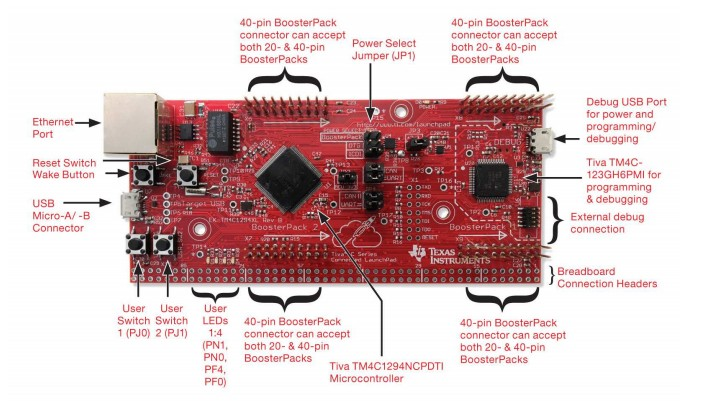
\includegraphics[width=.7\textwidth]{../images/tiva_tm4c1294}
  \caption{Microcontrolador empleado en el proyecto}
\end{figure}

Como se puede observar, ademas de poseer una conexion Ethernet, USB y una serie de leds, tendra un microcontrolador integrado, el Tiva TM123GH, conectado a un puerto USB cuya funcionalidad sera programar el microcontrolador principal. \\
Ademas de ello, dispone de dos pares de ristras de pines destinadas al conexionado de dos Boosterpacks distintos, de tal modo que se puedan ampliar las funcionalidades como pueden ser una pantalla o el boosterpack empleado en este proyecto, BOOSTXL-SENSORS. \\

Para conocer informacion adiccional sobre el microcontrolador implementado en la placa puede la guia propocionada por el fabricante: \url{http://www.ti.com/lit/ug/spmu365c/spmu365c.pdf}. \\

Se ha optado por el uso de este microcontrolador para este proyecto por su capacidad de .......... lo de poder controladr el raton........
\newpage

En cuanto al Boosterpack empleado, BOOSTXL-SENSORS, es el mostrado a continuacion: \\
\begin{figure}[h!]
 \centering
 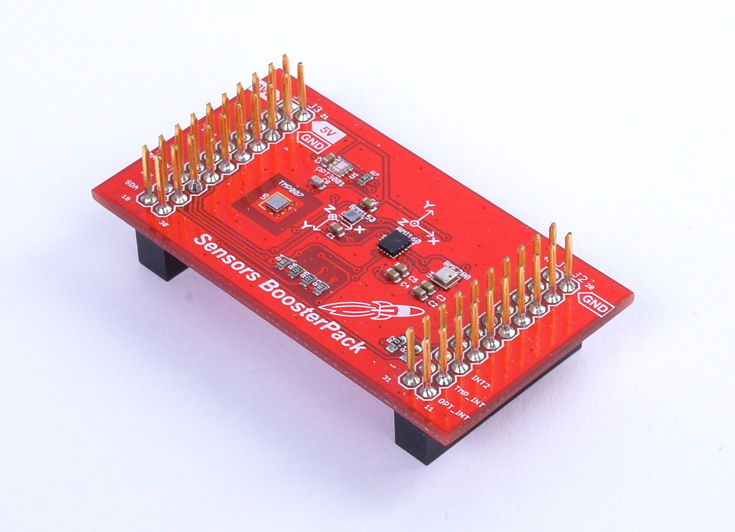
\includegraphics[width=.4\textwidth]{../images/sensors_bp}
 \caption{Boosterpack empleado en el proyecto}
\end{figure}

contiene una gran cantidad de sensores como son una IMU, un magnetometro, sensores ambiente y de luminosidad y sensor de temperatura. En lo que a este proyecto respecta, el principal sensor que se empleara sera la IMU integrada, la \textit{BMI160} de 6 ejes, es decir, se encuentra formada por un acelerometro de 3 ejes y un giroscopio de 3 ejes. \\

La medida del acelerometro sera dada en \textit{g}, la cual puede ser estimulada modificando la orientacion respecto a la gravedad de la tierra, o cambiando la velocidad a lo largo de un eje. En cuanto a la medida del giroscopio sera dada en grados por segundo, la cual se estimulara girando la placa respecto sus ejes absolutos. \\
En este proyecto, se emplearan las medidas asociadas a las velocidades angulares en torno a los ejes X y Z, ya que son las unicas empleadas para posicionarse en el plano 2D que forma la pantalla del computador. Se mostrara a continuacion una imagen en la cual se mostrara el movimento en torno al eje X que generara una variacion de la velocidad angular medida por el giroscpio:\\
\begin{figure}[h!]
 \centering
 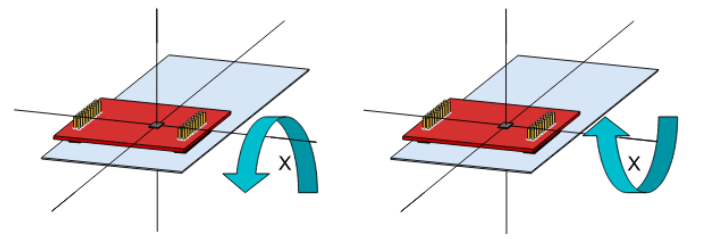
\includegraphics[width=.6\textwidth]{../images/mov_axisX_bmi}
 \caption{Movimento en torno al eje X que genera una variacion de velocidad angular}
\end{figure}

La variacion del angulo en torno al eje Z se medira del mismo modo, como se muestra a continuacion: \\
\begin{figure}[h!]
 \centering
 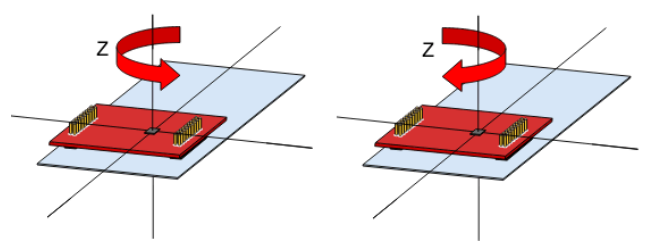
\includegraphics[width=.6\textwidth]{../images/mov_axisZ_bmi}
 \caption{Movimento en torno al eje Z que genera una variacion de velocidad angular}
\end{figure}

\newpage
La comunicacion del sensor con otros sensores del boosterpack y con la placa sera por medio de $I^2C$, el cual es el principal bus serie de datos, empleado para la comunicacion entre elementos de un circuito. \\

<<<<<<< HEAD
Al igual que antes, se puede consultar datos concretos de cada sensor en la guia proporcionada por el fabricante:
\url{http://www.ti.com/lit/ug/slau666b/slau666b.pdf}

\subsection{Descripcion del software empleado}
En cuanto al software empleado se basara en la API proporcionada por el fabricante, \textit{TivaWare} para la familia de microcontoladores TIVA. Esta API contiene los elementos que se muestran en la siguiente imagen:\\
\begin{figure}[h!]
 \centering
 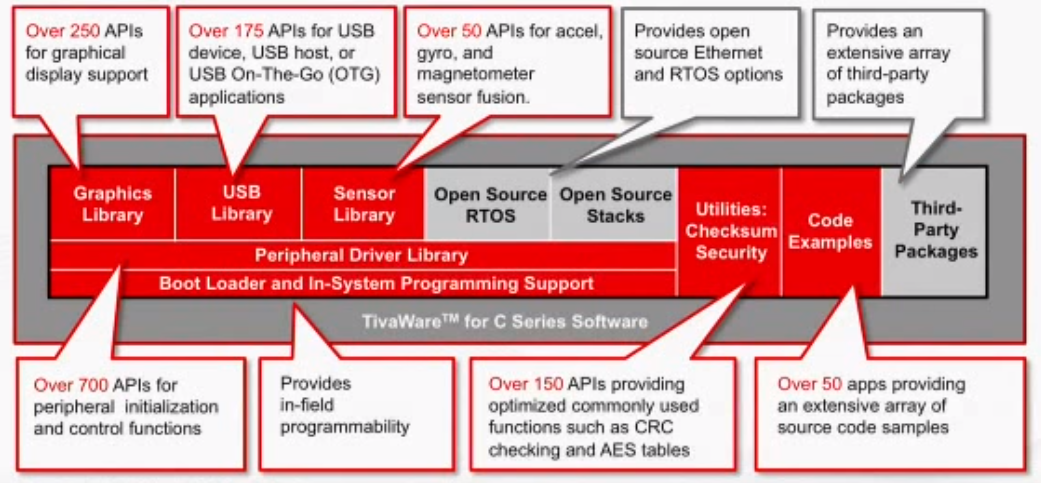
\includegraphics[width=.8\textwidth]{../images/tivaware_struct}
 \caption{Estructura de la API Tivaware}
\end{figure}
=======
\begin{verbatim}
# KeyPad Digilent Adept Conexions
#Input
Net gpio_keypad_GPIO_IO_I_pin<0> LOC=K12 | IOSTANDARD=LVCMOS33; #ROW4
Net gpio_keypad_GPIO_IO_I_pin<1> LOC=K13 | IOSTANDARD=LVCMOS33; #ROW3
Net gpio_keypad_GPIO_IO_I_pin<2> LOC=F17 | IOSTANDARD=LVCMOS33; #ROW2
Net gpio_keypad_GPIO_IO_I_pin<3> LOC=F18 | IOSTANDARD=LVCMOS33; #ROW1
#Output
Net gpio_keypad_GPIO2_IO_O_pin<0> LOC=H12 | IOSTANDARD=LVCMOS33; #COL4
Net gpio_keypad_GPIO2_IO_O_pin<1> LOC=G13 | IOSTANDARD=LVCMOS33; #COL3
Net gpio_keypad_GPIO2_IO_O_pin<2> LOC=E16 | IOSTANDARD=LVCMOS33; #COL2
Net gpio_keypad_GPIO2_IO_O_pin<3> LOC=E18 | IOSTANDARD=LVCMOS33; #COL1
\end{verbatim}

\begin{table}[h!]
    \centering
    \begin{tabular}{|l|l|l|l|}
    \hline
     &\multicolumn{1}{c|}{Instrucción} & {Operator Code} & {Descripción} \\
     \hline \hline
    \multirow{6}{*}{\textit{Load and Stores}} & LDA\_IMM  & x"86",<data> & Carga con direccionamiento inmediato \\ \cline{2-4}
                            								  & LDA\_DIR  & x"87",<addr> & Carga con direccionamiento directo \\ \cline{2-4}
                            								  & LDB\_IMM  & x"88",<data> & Carga con direccionamiento inmediato \\ \cline{2-4}
                            								  & LDB\_DIR  & x"89",<addr> & Carga con direccionamiento directo \\ \cline{2-4}
																						  & STA\_DIR  & x"96",<addr> & Almacena dato en registro A \\ \cline{2-4}
																							& STB\_DIR  & x"97",<addr> & Almacena dato en registro B \\ \cline{2-4}
																							\hline
	\multirow{8}{*}{\textit{Data Manipulations}} & ADD\_AB  & x"42" & A=A+B \\ \cline{2-4}
	                         								     & SUB\_AB  & x"43" & A=A-B \\ \cline{2-4}
																					  & AND\_AB  & x"44" &  A = A \& B \\ \cline{2-4}
																					  & OR\_AB  & x"45" &  A=A | B \\ \cline{2-4}
																						& INCA  & x"46" &   A=A+1 \\ \cline{2-4}
																						& INCB  & x"47" &  B=B+1 \\ \cline{2-4}
																						& DECA  & x"48" &  A=A-1 \\ \cline{2-4}
																						& DECB  & x"49" &  B=B-1 \\ \cline{2-4}
																							\hline
 \multirow{9}{*}{\textit{Branches}}  & BRA  & x"20",<addr> & Branch siempre \\ \cline{2-4}
                          					 & BMI  & x"21",<addr> & Branch si N=1 \\ \cline{2-4}
																		 & BPL  & x"22",<addr> & Branch si N=0 \\ \cline{2-4}
																		 & BEQ  & x"23",<addr> & Branch si Z=1 \\ \cline{2-4}
																	   & BNE  & x"24",<addr> & Branch si Z=0 \\ \cline{2-4}
																		 & BVS  & x"25",<addr> & Branch si V=1 \\ \cline{2-4}
																		 & BVC  & x"26",<addr> & Branch si V=0 \\ \cline{2-4}
																		 & BCS  & x"27",<addr> & Branch si C=1 \\ \cline{2-4}
																	   & BCC  & x"28",<addr> & Branch si C=0 \\ \cline{2-4}
																		 	\hline
    \end{tabular}    \caption{Set de instrucciones del microprocesador}
    \end{table}

>>>>>>> 94616271741b9c70a6ba9afa412b2d6454d5cee5

Principalmente, se emplearan las liberias asociadas al manejo de los perifericos, \textit{Peripheral Driver Library}, al manejo del puerto USB,\textit{USB Library} y al manejo de sensores,\textit{Sensor Library}. \\
Ademas de la gran ayuda brinda la API, se proporcionan una serie de ejemplos de uso que ayudaran al desarrollo del software propio. \\

Ademas de ello, ha sido necesario el uso de librerias para el manejo de los GPio de la placa y la comunicacion por el puerto serie de la UART. \\
Ademas de ello, se han empleado una serie de declaraciones proporciondadas por el profesor para solventar el desajuste de la actualizacion de las librerias, \textit{driverlib2.h} y \textit{sensorlib2.h}.

\newpage
\section{Funcionamiento del proyecto}
En cuando ...

\section{Código de programación desarrollado}

\newpage
\section{Posibles mejoras del proyecto}
En cuando a la principal mejora del proyecto, se basara en la implementacion de una comunicacion inalambrica en el mismo. Durante el desarrollo del proyecto se plantearon diversas vias posibles de implementacion:
\begin{itemize}
\item Implementacion de una comunicacion basada en radio-frecuencia. Esta via se planteo empleando el boosterpack del fabricante \textit{Texas Instrument}, CC110L, el cual emplea el protocolo de comunicacion SimpliciTI. Sin embargo, este modulo de radio frecuencia, ha sido disenado para su utilizacion con el microcontrolador MSP430, y es poco compatible con otros microcontroladores, aunque sea del mismo fabricante. \\
\begin{figure}[h!]
 \centering
 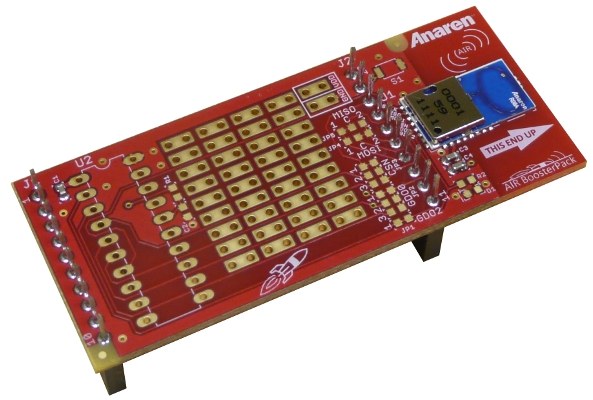
\includegraphics[width=.3\textwidth]{../images/rf_bp}
 \caption{430BOOST-CC110L Boosterpack}
\end{figure}

\item Implementacion de una comunicacion Wi-Fi. Para la implementacion de este modo de comunicacion, se haria uso del modulo ESP01, el cual es un modulo Wi-Fi de bajo coste, que puede ser configurado como punto de acceso o como cliente y enviar mensajes TCP entre varios para comunicarse entre ellos. \\
\begin{figure}[h!]
 \centering
 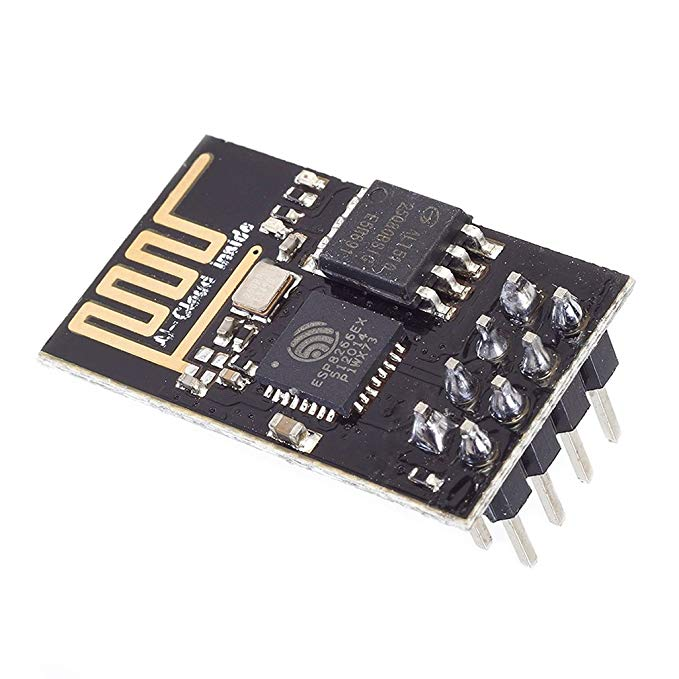
\includegraphics[width=.2\textwidth]{../images/esp8266}
 \caption{Modulo WiFi ESP01}
\end{figure}
\end{itemize}

Esta ultima via de comunicacion, es la que se ha considerado mas factible ya que los modulos ESP01 emplean comandos AT, es decir, el conjunto de comandos Hayes, los cuales son un conjunto de comandos empleados para configurar y parametrizar los modems. \\
Debido a que la comunicacion con el ESP01 es UART, para establecer una comunicacion con `el seria necesario, ademas de todo el entramado de conexiones de red, enviar comandos por comunicacion serial. Sin embargo, no se ha optado por implementarlo en este proyecto, debido a la necesidad del uso de los objetos inherentes al lenguaje de programacion C++ y sus clases.

\newpage
\section{Anexos}


\begin{lstlisting}[language=C,style=CStyle, caption={Declaración e inicialización de variables}]

\end{lstlisting}
\end{document}
